\section{Introduction to Deep Survival Machines}

Deep Survival Machines (DSM) \parencite{nagpal2021dsm} represents a paradigm shift in survival analysis, introducing a novel approach that bridges the gap between traditional statistical methods and modern deep learning. This chapter explores how DSM combines the strengths of neural networks with parametric survival modeling to overcome the limitations of both conventional approaches \parencite{cox1972,kaplan1958} and earlier neural network adaptations for survival analysis \parencite{katzman2018,chapfuwa2018}.

\begin{notebox}[title=Chapter Overview]
This chapter covers:
\begin{itemize}
    \item The limitations of traditional survival analysis methods
    \item Complex hazard patterns in real-world survival data
    \item The conceptual innovation of the DSM mixture approach
    \item Mathematical foundations of DSM
    \item Implementation details and practical considerations
    \item Advantages of DSM over alternative methods
    \item Applications and results in real-world scenarios
\end{itemize}
\end{notebox}

\section{Limitations of Traditional Survival Analysis Methods}

Despite the theoretical foundations discussed in the previous chapter, traditional survival analysis methods face significant limitations when applied to complex, high-dimensional real-world data. Understanding these limitations provides the motivation for developing more advanced approaches like Deep Survival Machines.

\subsection{Limitations of Non-parametric Methods}

The Kaplan-Meier estimator and other non-parametric methods, while making minimal assumptions about the underlying distribution, have several important constraints:

\begin{itemize}
    \item \textbf{Limited covariate handling:} They cannot effectively incorporate continuous covariates or high-dimensional feature spaces
    \item \textbf{Reliance on stratification:} Covariate adjustment is limited to stratification by categorical variables, which quickly becomes impractical with multiple variables
    \item \textbf{No extrapolation:} Predictions cannot extend beyond the largest observed event time in the dataset
    \item \textbf{Curse of dimensionality:} Performance degrades in high-dimensional settings
    \item \textbf{Inefficient use of data:} Cannot leverage patterns across different strata
\end{itemize}

\subsection{Limitations of the Cox Proportional Hazards Model}

While the Cox model addresses some limitations of non-parametric methods by enabling covariate adjustment, it introduces its own constraints:

\begin{itemize}
    \item \textbf{Proportional hazards assumption:} Assumes that the hazard ratio between any two subjects remains constant over time—an assumption frequently violated in practice
    \item \textbf{Linear effects:} Assumes that covariates have a log-linear effect on the hazard, which may not capture complex non-linear relationships
    \item \textbf{Baseline hazard challenges:} The baseline hazard estimation is often unstable, especially with sparse data at longer follow-up times
    \item \textbf{Time-varying effects:} Accommodating time-varying covariate effects requires complex model extensions
    \item \textbf{Limited interaction modeling:} Capturing complex interactions between covariates requires explicit specification
\end{itemize}

\subsection{Limitations of Early Neural Network Adaptations}

Early efforts to apply neural networks to survival analysis, while promising, retained significant limitations:

\begin{itemize}
    \item \textbf{Specialized architectures:} Required complex, specialized architectures to handle censored data
    \item \textbf{Proportional hazards heritage:} Many approaches still relied on the proportional hazards assumption
    \item \textbf{Black-box nature:} Limited interpretability and uncertainty quantification
    \item \textbf{Numerical challenges:} Suffered from instability in optimization and prediction
    \item \textbf{Distribution constraints:} Often still constrained to specific parametric forms or semi-parametric assumptions
\end{itemize}

These limitations highlight the need for a more flexible approach that can leverage the representational power of neural networks while respecting the unique characteristics of survival data.

\section{Complex Hazard Patterns in Real-World Data}

Real-world survival data often exhibits complex hazard patterns that cannot be adequately captured by traditional models, which typically assume simple monotonic hazard functions.

\subsection{Multi-Modal Hazard Functions}

Many real-world processes, particularly in medicine, show hazard patterns with multiple modes or complex shapes:

\begin{itemize}
    \item \textbf{Early high risk followed by plateau:} Common in post-surgical scenarios where immediate complications dominate early risk
    \item \textbf{Delayed risk that increases over time:} Seen in certain cancers where recurrence risk grows after an initial treatment response
    \item \textbf{Multiple risk peaks (biphasic patterns):} Observed in diseases with distinct phases, such as certain autoimmune conditions
    \item \textbf{Risk patterns that vary by subpopulation:} Different risk profiles for different patient subgroups, even after controlling for observable covariates
\end{itemize}

\begin{figure}[htbp]
    \centering
    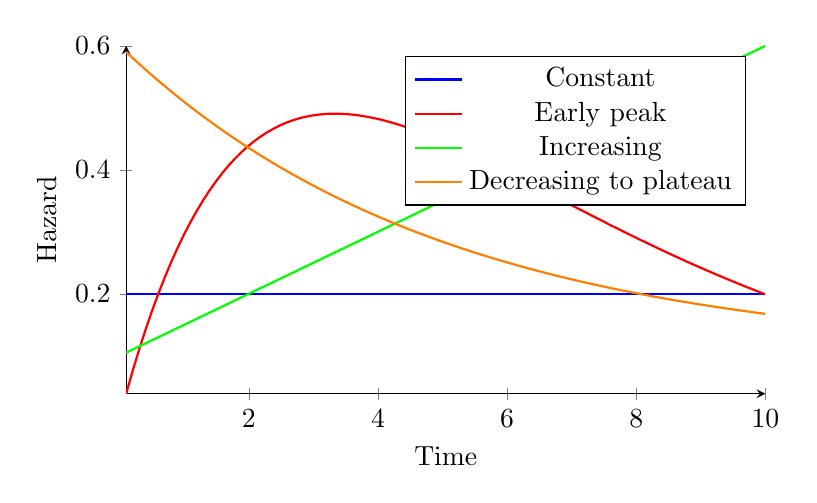
\begin{tikzpicture}
        \begin{axis}[
            width=0.8\textwidth,
            height=6cm,
            xlabel={Time},
            ylabel={Hazard},
            axis lines=left,
            domain=0.1:10,
            samples=100,
            legend pos=north east,
            ]
            % Different hazard shapes
            \addplot[blue, thick] {0.2}; % Constant
            \addplot[red, thick] {0.4*x*exp(-0.3*x)}; % Hump
            \addplot[green, thick] {0.1 + 0.05*x}; % Increasing
            \addplot[orange, thick] {0.5*exp(-0.2*x) + 0.1}; % Decreasing to plateau
            \legend{Constant, Early peak, Increasing, Decreasing to plateau}
        \end{axis}
    \end{tikzpicture}
    \caption{Examples of different hazard patterns observed in real-world survival data. Traditional models often assume a single pattern (such as constant or monotonically increasing/decreasing), but real processes frequently exhibit more complex behavior.}
    \label{fig:dsm-hazard-patterns}
\end{figure}

\subsection{The Need for Uncertainty Quantification}

Another critical limitation of many survival analysis methods is the lack of robust uncertainty quantification, which is essential in high-stakes decision-making contexts.

\begin{examplebox}[title=Clinical Decision-Making with Uncertainty]
Consider a physician deciding between aggressive and conservative treatment for a cancer patient:
\begin{itemize}
    \item A point estimate suggesting 60\% 5-year survival probability provides limited guidance
    \item Knowing the confidence interval is 40-80\% indicates substantial uncertainty
    \item This uncertainty information might lead to additional testing or consideration of patient preferences
    \item Without proper uncertainty quantification, decision-makers may have false confidence in predictions
\end{itemize}
\end{examplebox}

Two fundamental types of uncertainty need to be addressed:
\begin{itemize}
    \item \textbf{Epistemic uncertainty:} Uncertainty due to model limitations and finite data—can theoretically be reduced with more data or better models
    \item \textbf{Aleatoric uncertainty:} Inherent randomness in the process being modeled—cannot be reduced with more data and represents genuine outcome variability
\end{itemize}

\begin{figure}[htbp]
    \centering
    \begin{tikzpicture}
        \begin{axis}[
            width=0.8\textwidth,
            height=6cm,
            xlabel={Time},
            ylabel={Survival Probability},
            axis lines=left,
            domain=0:10,
            samples=100,
            ]
            % Mean prediction
            \addplot[blue, thick] {exp(-(x/5)^1.2)};
            
            % Upper and lower confidence bounds with named paths
            \addplot[blue, dashed, name path=upper] {exp(-(x/6)^1.2)};
            \addplot[blue, dashed, name path=lower] {exp(-(x/4)^1.2)};
            
            % Fill between the named paths
            \addplot[blue!20, forget plot] fill between[of=upper and lower];
            
            \legend{Mean Prediction, Uncertainty Bounds}
        \end{axis}
    \end{tikzpicture}
    \caption{Survival curve with uncertainty bounds. The shaded region represents the uncertainty in the survival estimates, which increases over time as less information is available. This visualization provides decision-makers with both the point estimate and a measure of confidence in that estimate.}
    \label{fig:survival-uncertainty}
\end{figure}

These complex hazard patterns and the need for robust uncertainty quantification motivate the development of more flexible and expressive approaches to survival analysis.

\section{Deep Survival Machines: Core Conceptual Innovation}

Deep Survival Machines introduces a novel approach to survival analysis that addresses the limitations of traditional methods while leveraging the representational power of neural networks.

\subsection{The Mixture Distribution Approach}

The central innovation of DSM is to model survival as a mixture of parametric distributions:

\begin{itemize}
    \item \textbf{Mixture composition:} The survival function is modeled as a weighted sum of multiple parametric survival functions
    \item \textbf{Component diversity:} Each component can capture a different risk pattern or represent a different subpopulation
    \item \textbf{Neural parameter mapping:} Neural networks learn to map from input features to distribution parameters and mixture weights
    \item \textbf{Flexible hazard representation:} The mixture approach can represent virtually any smooth hazard function
    \item \textbf{Natural uncertainty quantification:} The mixture variance provides a measure of predictive uncertainty
\end{itemize}

\begin{figure}[htbp]
    \centering
    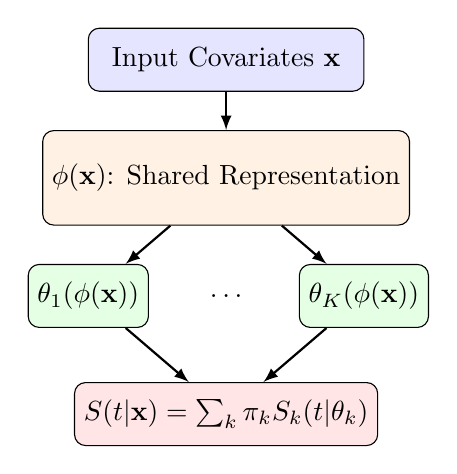
\begin{tikzpicture}[scale=1.0, transform shape]
        \node[draw, rounded corners, minimum width=3.5cm, minimum height=0.8cm, fill=blue!10] (input) at (0,0) {Input Covariates $\mathbf{x}$};
        
        \node[draw, rounded corners, minimum width=3.5cm, minimum height=1.2cm, fill=orange!10] (shared) at (0,-1.5) {$\phi(\mathbf{x})$: Shared Representation};
        
        \node[draw, rounded corners, minimum width=1.5cm, minimum height=0.8cm, fill=green!10] (k1) at (-1.75,-3) {$\theta_1(\phi(\mathbf{x}))$};
        \node at (0,-3) {$\ldots$};
        \node[draw, rounded corners, minimum width=1.5cm, minimum height=0.8cm, fill=green!10] (k2) at (1.75,-3) {$\theta_K(\phi(\mathbf{x}))$};
        
        \node[draw, rounded corners, minimum width=3.5cm, minimum height=0.8cm, fill=red!10] (output) at (0,-4.5) {$S(t|\mathbf{x}) = \sum_k \pi_k S_k(t|\theta_k)$};
        
        \draw[-latex, thick] (input) -- (shared);
        \draw[-latex, thick] (shared) -- (k1);
        \draw[-latex, thick] (shared) -- (k2);
        \draw[-latex, thick] (k1) -- (output);
        \draw[-latex, thick] (k2) -- (output);
    \end{tikzpicture}
    \caption{Conceptual architecture of Deep Survival Machines. Input covariates are processed through a shared representation layer, which then feeds into parameter networks for each mixture component. The final survival function is a weighted combination of the component survival functions.}
    \label{fig:dsm-architecture}
\end{figure}

\subsection{Architectural Components}

The DSM architecture consists of three main components that work together to create a flexible and expressive survival model:

\subsubsection{Representation Network}

The representation network transforms raw covariates into a latent feature representation:
\begin{itemize}
    \item Can use any neural network architecture appropriate for the data type (MLP for tabular data, CNN for images, transformers for sequential data, etc.)
    \item Learns task-relevant feature extraction and transformation
    \item Enables automatic feature learning and extraction of complex patterns
    \item Creates a shared representation that feeds into the parameter networks
\end{itemize}

\subsubsection{Mixture Model}

The mixture model combines multiple parametric survival distributions:
\begin{itemize}
    \item Typically uses 2-8 components, depending on data complexity
    \item Components are usually from the same parametric family (e.g., all Weibull) but with different parameters
    \item Models different risk patterns and subpopulations implicitly discovered from the data
    \item Creates a flexible composition that can represent complex hazard shapes
\end{itemize}

\subsubsection{Parameter Networks}

Parameter networks map from the shared representation to the parameters of each distribution component:
\begin{itemize}
    \item Separate networks for each parameter type (e.g., shape, scale) and each component
    \item Include constraints to ensure valid parameter ranges (e.g., positive shape parameters)
    \item Learn adaptive mixture weights that determine the contribution of each component
    \item Enable personalized parameter estimation based on individual covariates
\end{itemize}

\section{Key Innovations of Deep Survival Machines}

Deep Survival Machines introduces several key innovations that distinguish it from both traditional survival methods and earlier neural network approaches.

\subsection{End-to-End Learning}

Unlike many traditional survival models that separate feature engineering from survival modeling, DSM enables end-to-end learning:
\begin{itemize}
    \item Joint optimization of representation learning and survival parameter estimation
    \item No need for separate feature engineering or transformation steps
    \item Gradient-based optimization of all model components
    \item Representation automatically adapts to the survival prediction task
\end{itemize}

\subsection{Flexible Hazard Modeling}

The mixture approach enables modeling of complex hazard patterns without restrictive assumptions:
\begin{itemize}
    \item No proportional hazards assumption required
    \item Can model virtually any survival distribution
    \item Automatically captures non-linear relationships between covariates and survival
    \item Adapts to the underlying data-generating process
\end{itemize}

\subsection{Uncertainty Quantification}

DSM provides natural uncertainty quantification through its mixture formulation:
\begin{itemize}
    \item The mixture variance provides a measure of predictive uncertainty
    \item Different components can represent different risk scenarios
    \item Uncertainty can be visualized through prediction intervals
    \item Both epistemic and aleatoric uncertainty are captured
\end{itemize}

\subsection{Risk Prediction Capabilities}

Unlike many survival models that focus on relative risks, DSM provides comprehensive risk assessment:
\begin{itemize}
    \item Direct probability outputs (not just relative risks)
    \item Time-dependent risk assessment at any time point
    \item Personalized survival curves for individual subjects
    \item Risk stratification based on predicted outcomes
\end{itemize}

\section{Mathematical Foundation of Deep Survival Machines}

To fully understand DSM, we need to examine its mathematical formulation, starting with the basic survival analysis functions and extending to the mixture framework.

\subsection{Survival Analysis Fundamentals: A Brief Recap}

As discussed in the previous chapter, for a random variable $T$ representing survival time, the key probability functions are:

\begin{equationbox}[title=Core Survival Functions]
\begin{align}
    \text{Survival function: } & S(t) = P(T > t) \\
    \text{CDF: } & F(t) = P(T \leq t) = 1 - S(t) \\
    \text{PDF: } & f(t) = \frac{d}{dt}F(t) = -\frac{d}{dt}S(t) \\
    \text{Hazard function: } & h(t) = \frac{f(t)}{S(t)} = -\frac{d}{dt}\log S(t) \\
    \text{Cumulative hazard: } & H(t) = \int_0^t h(u) du = -\log S(t)
\end{align}
\end{equationbox}

These functions are interrelated, and each provides a different perspective on the time-to-event process. DSM builds on this foundation by introducing a mixture framework.

\subsection{The Mixture Framework}

The fundamental insight of DSM is to model the survival distribution as a mixture of parametric distributions:

\begin{equationbox}[title=DSM Mixture Survival Function]
\begin{align}
    S(t|\mathbf{x}) &= \sum_{k=1}^{K} \pi_k(\mathbf{x}) S_k(t|\mathbf{x})
\end{align}

where:
\begin{itemize}
    \item $S(t|\mathbf{x})$ is the overall survival function given covariates $\mathbf{x}$
    \item $S_k(t|\mathbf{x})$ is the survival function for the $k$-th component
    \item $\pi_k(\mathbf{x})$ is the mixture weight for the $k$-th component
    \item $\sum_{k=1}^K \pi_k(\mathbf{x}) = 1$ and $\pi_k(\mathbf{x}) \geq 0$ for all $k$
\end{itemize}
\end{equationbox}

From this mixture survival function, we can derive the corresponding density and hazard functions:

\begin{equationbox}[title=DSM Mixture Density and Hazard]
\begin{align}
    f(t|\mathbf{x}) &= -\frac{d}{dt}S(t|\mathbf{x}) = \sum_{k=1}^{K} \pi_k(\mathbf{x}) f_k(t|\mathbf{x}) \\
    h(t|\mathbf{x}) &= \frac{f(t|\mathbf{x})}{S(t|\mathbf{x})} = \frac{\sum_{k=1}^{K} \pi_k(\mathbf{x}) f_k(t|\mathbf{x})}{\sum_{k=1}^{K} \pi_k(\mathbf{x}) S_k(t|\mathbf{x})}
\end{align}
\end{equationbox}

\subsection{Insight into Hazard Composition}

The mixture hazard can be rewritten to provide insight into how the different components contribute:

\begin{equationbox}[title=Alternative Hazard Formulation]
\begin{align}
    h(t|\mathbf{x}) &= \frac{\sum_{k=1}^{K} \pi_k(\mathbf{x}) f_k(t|\mathbf{x})}{\sum_{k=1}^{K} \pi_k(\mathbf{x}) S_k(t|\mathbf{x})} \\
    &= \sum_{k=1}^{K} \frac{\pi_k(\mathbf{x}) S_k(t|\mathbf{x})}{\sum_{j=1}^{K} \pi_j(\mathbf{x}) S_j(t|\mathbf{x})} h_k(t|\mathbf{x})
\end{align}
\end{equationbox}

This reveals that the overall hazard is a weighted combination of component hazards, where the weights change over time. The weighting factor $\frac{\pi_k S_k}{\sum_j \pi_j S_j}$ represents the posterior probability that an individual who survived to time $t$ belongs to component $k$.

\section{Parametric Component Distributions}

DSM can use various parametric distributions for its mixture components. The two most common choices are the Weibull and log-normal distributions.

\subsection{Weibull Distribution}

The Weibull distribution is frequently used due to its flexibility in modeling different hazard shapes:

\begin{equationbox}[title=Weibull Distribution Functions]
\begin{align}
    S_k(t|\mathbf{x}) &= \exp\left[-\left(\frac{t}{\lambda_k(\mathbf{x})}\right)^{\alpha_k(\mathbf{x})}\right] \\
    f_k(t|\mathbf{x}) &= \frac{\alpha_k(\mathbf{x})}{\lambda_k(\mathbf{x})}\left(\frac{t}{\lambda_k(\mathbf{x})}\right)^{\alpha_k(\mathbf{x})-1}\exp\left[-\left(\frac{t}{\lambda_k(\mathbf{x})}\right)^{\alpha_k(\mathbf{x})}\right] \\
    h_k(t|\mathbf{x}) &= \frac{\alpha_k(\mathbf{x})}{\lambda_k(\mathbf{x})}\left(\frac{t}{\lambda_k(\mathbf{x})}\right)^{\alpha_k(\mathbf{x})-1}
\end{align}

where:
\begin{itemize}
    \item $\lambda_k(\mathbf{x})$ is the scale parameter, which influences the median survival time
    \item $\alpha_k(\mathbf{x})$ is the shape parameter, which determines the hazard behavior
\end{itemize}
\end{equationbox}

The shape parameter $\alpha_k$ controls the hazard shape in a Weibull distribution:
\begin{itemize}
    \item $\alpha_k = 1$: Constant hazard (exponential distribution)
    \item $\alpha_k > 1$: Increasing hazard (e.g., wear-out, aging)
    \item $\alpha_k < 1$: Decreasing hazard (e.g., early failures, infections)
\end{itemize}

\begin{figure}[htbp]
    \centering
    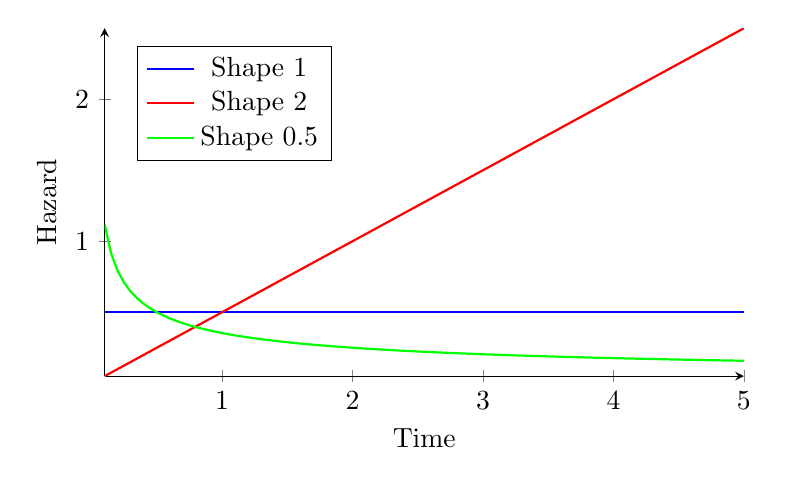
\begin{tikzpicture}
        \begin{axis}[
            width=0.8\textwidth,
            height=6cm,
            xlabel={Time},
            ylabel={Hazard},
            axis lines=left,
            domain=0.1:5,
            samples=100,
            legend style={at={(0.05,0.95)}, anchor=north west},
            ]
            \addplot[blue, thick] {1/2};
            \addplot[red, thick] {2/2*(x/2)^1};
            \addplot[green, thick] {0.25/sqrt(x/2)};
            \legend{Shape 1, Shape 2, Shape 0.5}
        \end{axis}
    \end{tikzpicture}
    \caption{Weibull hazard functions with different shape parameters. When $\alpha = 1$ (blue), the hazard is constant. When $\alpha > 1$ (red), the hazard increases with time. When $\alpha < 1$ (green), the hazard decreases with time.}
    \label{fig:weibull-hazards}
\end{figure}

\subsection{Log-Normal Distribution}

DSM can also use log-normal components, which provide different hazard characteristics:

\begin{equationbox}[title=Log-Normal Distribution Functions]
\begin{align}
    S_k(t|\mathbf{x}) &= 1 - \Phi\left(\frac{\log t - \mu_k(\mathbf{x})}{\sigma_k(\mathbf{x})}\right) \\
    f_k(t|\mathbf{x}) &= \frac{1}{t\sigma_k(\mathbf{x})\sqrt{2\pi}}\exp\left(-\frac{(\log t - \mu_k(\mathbf{x}))^2}{2\sigma_k^2(\mathbf{x})}\right) \\
    h_k(t|\mathbf{x}) &= \frac{f_k(t|\mathbf{x})}{S_k(t|\mathbf{x})}
\end{align}

where:
\begin{itemize}
    \item $\mu_k(\mathbf{x})$ is the location parameter
    \item $\sigma_k(\mathbf{x})$ is the scale parameter
    \item $\Phi$ is the standard normal cumulative distribution function
\end{itemize}
\end{equationbox}

The log-normal distribution has distinct characteristics:
\begin{itemize}
    \item Non-monotonic hazard that increases and then decreases
    \item Better for modeling certain diseases with delayed effects
    \item More parameters to optimize
    \item Often used for modeling cancer survival with delayed treatment effects
\end{itemize}

\subsection{The Power of Mixtures}

The mixture approach allows DSM to model complex hazard patterns that would be impossible with a single parametric distribution. With just 2-4 components, DSM can represent:

\begin{itemize}
    \item Bathtub hazards (high early risk, low middle, high late)
    \item Multi-modal hazards (multiple risk peaks)
    \item U-shaped hazards
    \item Virtually any smooth hazard function
\end{itemize}

\begin{figure}[htbp]
    \centering
    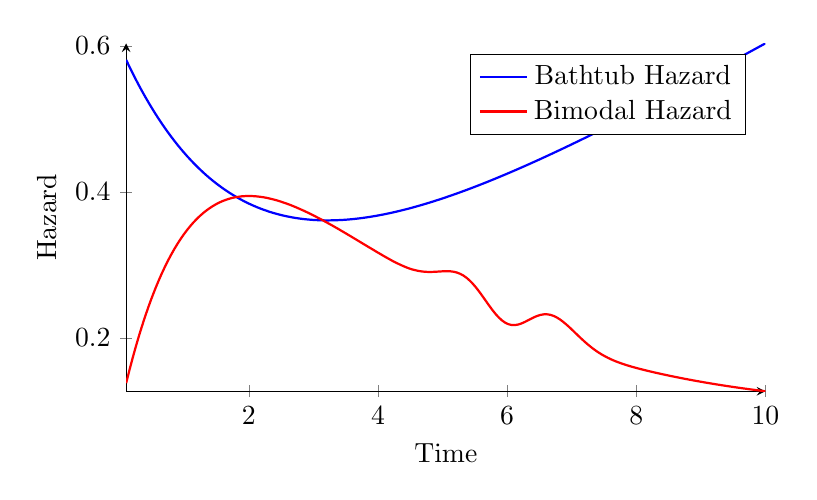
\begin{tikzpicture}
        \begin{axis}[
            width=0.8\textwidth,
            height=6cm,
            xlabel={Time},
            ylabel={Hazard},
            axis lines=left,
            domain=0.1:10,
            samples=200,
            legend pos=north east,
            ]
            % Bathtub hazard (high early, low middle, rising late)
            \addplot[blue, thick] {0.5*exp(-0.5*x) + 0.05*x + 0.1};
            
            % Bimodal hazard (two peaks)
            \addplot[red, thick] {0.4*x*exp(-0.5*x) + 0.2*(x-6)^2*exp(-2*(x-6)^2) + 0.1};
            
            \legend{Bathtub Hazard, Bimodal Hazard}
        \end{axis}
    \end{tikzpicture}
    \caption{Complex hazard patterns that can be modeled using mixtures of simple parametric distributions. The bathtub pattern (blue) shows high initial risk, followed by a stable period, and then increasing risk. The bimodal pattern (red) shows two distinct risk peaks.}
    \label{fig:complex-hazards}
\end{figure}

\section{Neural Parameter Mapping}

A key aspect of DSM is the use of neural networks to map from input features to distribution parameters.

\subsection{From Features to Distribution Parameters}

DSM employs a series of neural network transformations to derive distribution parameters from input features:

\begin{equationbox}[title=Neural Parameter Mapping]
\begin{align}
    \phi(\mathbf{x}) &= \text{neural\_network}(\mathbf{x}) \\
    \alpha_k(\mathbf{x}) &= \text{softplus}(w_{\alpha_k}^T \phi(\mathbf{x}) + b_{\alpha_k}) + \varepsilon \\
    \lambda_k(\mathbf{x}) &= \text{softplus}(w_{\lambda_k}^T \phi(\mathbf{x}) + b_{\lambda_k}) + \varepsilon \\
    \tilde{\pi}_k(\mathbf{x}) &= w_{\pi_k}^T \phi(\mathbf{x}) + b_{\pi_k} \\
    \pi_k(\mathbf{x}) &= \frac{\exp(\tilde{\pi}_k(\mathbf{x}))}{\sum_{j=1}^{K} \exp(\tilde{\pi}_j(\mathbf{x}))}
\end{align}

where:
\begin{itemize}
    \item $\phi(\mathbf{x})$ is the shared representation from the neural network
    \item $w_{\alpha_k}$, $w_{\lambda_k}$, $w_{\pi_k}$ are parameter-specific weights
    \item $b_{\alpha_k}$, $b_{\lambda_k}$, $b_{\pi_k}$ are parameter-specific biases
    \item softplus activation ensures positive values for $\alpha_k$ and $\lambda_k$
    \item softmax ensures mixture weights $\pi_k$ sum to 1
    \item $\varepsilon$ is a small positive constant (e.g., 0.01) to prevent numerical issues
\end{itemize}
\end{equationbox}

\subsection{Network Architecture}

The complete DSM architecture can be visualized as follows:

\begin{figure}[htbp]
    \centering
    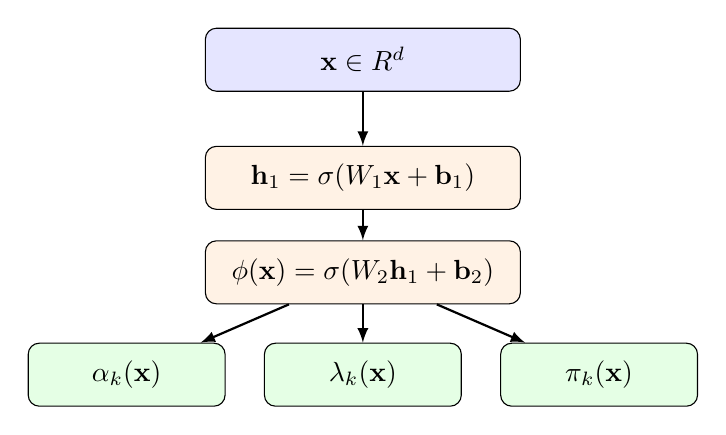
\begin{tikzpicture}
        \node[draw, rounded corners, minimum width=4cm, minimum height=0.8cm, fill=blue!10] (input) at (0,0) {$\mathbf{x} \in \mathbb{R}^d$};
        
        \node[draw, rounded corners, minimum width=4cm, minimum height=0.8cm, fill=orange!10] (hidden1) at (0,-1.5) {$\mathbf{h}_1 = \sigma(W_1\mathbf{x} + \mathbf{b}_1)$};
        
        \node[draw, rounded corners, minimum width=4cm, minimum height=0.8cm, fill=orange!10] (hidden2) at (0,-2.7) {$\phi(\mathbf{x}) = \sigma(W_2\mathbf{h}_1 + \mathbf{b}_2)$};
        
        \node[draw, rounded corners, minimum width=2.5cm, minimum height=0.8cm, fill=green!10] (alpha) at (-3,-4) {$\alpha_k(\mathbf{x})$};
        
        \node[draw, rounded corners, minimum width=2.5cm, minimum height=0.8cm, fill=green!10] (lambda) at (0,-4) {$\lambda_k(\mathbf{x})$};
        
        \node[draw, rounded corners, minimum width=2.5cm, minimum height=0.8cm, fill=green!10] (pi) at (3,-4) {$\pi_k(\mathbf{x})$};
        
        \draw[-latex, thick] (input) -- (hidden1);
        \draw[-latex, thick] (hidden1) -- (hidden2);
        \draw[-latex, thick] (hidden2) -- (alpha);
        \draw[-latex, thick] (hidden2) -- (lambda);
        \draw[-latex, thick] (hidden2) -- (pi);
    \end{tikzpicture}
    \caption{Neural network architecture for DSM. Input features are processed through shared hidden layers to create a representation $\phi(\mathbf{x})$, which is then fed into parameter-specific output heads to generate distribution parameters and mixture weights.}
    \label{fig:dsm-network}
\end{figure}

\section{Training Deep Survival Machines}

Training DSM involves defining an appropriate loss function and addressing several numerical challenges.

\subsection{Loss Function Formulation}

For censored survival data:
\begin{itemize}
    \item If event observed ($\delta_i = 1$): Time $t_i$ is the exact event time
    \item If censored ($\delta_i = 0$): Event occurs after $t_i$ (right censoring)
\end{itemize}

The likelihood contribution for each observation is:
\begin{align}
    L_i = [f(t_i|\mathbf{x}_i)]^{\delta_i} \cdot [S(t_i|\mathbf{x}_i)]^{1-\delta_i}
\end{align}

Taking the negative log of the likelihood and expanding:
\begin{align}
    -\log L_i &= -\delta_i \log f(t_i|\mathbf{x}_i) - (1-\delta_i) \log S(t_i|\mathbf{x}_i) \\
    &= -\delta_i \log \left[\sum_{k=1}^{K} \pi_k(\mathbf{x}_i) f_k(t_i|\mathbf{x}_i)\right] \\
    &\quad - (1-\delta_i) \log \left[\sum_{k=1}^{K} \pi_k(\mathbf{x}_i) S_k(t_i|\mathbf{x}_i)\right]
\end{align}

The full loss is then the sum over all observations:
\begin{align}
    \mathcal{L}_{DSM} = \sum_{i=1}^N -\log L_i
\end{align}

\subsection{ELBO-Based Regularization}

Mixture models can suffer from component collapse, where all weight concentrates in just one component. To encourage the use of multiple components and create more diverse representations, DSM employs an Evidence Lower Bound (ELBO) regularization approach.

From a latent variable perspective, we can view $k$ as a latent mixture component:
\begin{align}
    \log p(t|\mathbf{x}) &= \log \sum_{k=1}^K p(t, k|\mathbf{x}) = \log \sum_{k=1}^K p(t|k,\mathbf{x})p(k|\mathbf{x}) \\
    &\geq \sum_{k=1}^K q(k|\mathbf{x}) \log \frac{p(t|k,\mathbf{x})p(k|\mathbf{x})}{q(k|\mathbf{x})} \\
    &= \sum_{k=1}^K q(k|\mathbf{x}) \log p(t|k,\mathbf{x}) - \sum_{k=1}^K q(k|\mathbf{x}) \log \frac{q(k|\mathbf{x})}{p(k|\mathbf{x})} \\
    &= \mathbb{E}_{q(k|\mathbf{x})}[\log p(t|k,\mathbf{x})] - KL(q(k|\mathbf{x})||p(k|\mathbf{x}))
\end{align}

If we use a uniform prior $p(k|\mathbf{x}) = 1/K$, the KL term becomes:
\begin{align}
    KL(q(k|\mathbf{x})||p(k|\mathbf{x})) = \sum_{k=1}^K q(k|\mathbf{x}) \log(K \cdot q(k|\mathbf{x}))
\end{align}

This motivates the ELBO regularizer that encourages diverse component usage:
\begin{align}
    \mathcal{L}_{ELBO} = \mathcal{L}_{DSM} + \beta \cdot KL(\pi(\mathbf{x})||\text{Uniform})
\end{align}

Where:
\begin{itemize}
    \item $\beta$ is a hyperparameter controlling regularization strength
    \item $\pi(\mathbf{x})$ is used as the $q(k|\mathbf{x})$ distribution
    \item This pushes mixture weights toward a uniform distribution
\end{itemize}

\section{Implementation Challenges and Solutions}

Implementing DSM involves addressing several numerical challenges to ensure stability and good performance.

\subsection{Numerical Stability Challenges}

The mixture likelihood calculation can encounter several numerical issues:
\begin{itemize}
    \item Overflow/underflow in exponential calculations
    \item Division by zero risk in hazard calculations
    \item Gradient explosion during backpropagation
    \item Parameter values spanning many orders of magnitude
\end{itemize}

\subsection{Log-Sum-Exp Trick}

For stable computation of $\log \sum_i e^{x_i}$, the log-sum-exp trick is essential:
\begin{align}
    \log \sum_i e^{x_i} &= \log \left[ e^a \sum_i e^{x_i - a}\right] \\
    &= a + \log \sum_i e^{x_i - a}
\end{align}
where $a = \max_i x_i$

This avoids underflow/overflow by bringing values to a numerically stable range.

\subsection{Gradient Detachment Strategy}

The gradient of the Weibull hazard with respect to the shape parameter $\alpha$ can explode for small time values when $\alpha < 1$:
\begin{align}
    \frac{\partial h(t|\alpha, \lambda)}{\partial \alpha} &= \frac{\partial}{\partial \alpha}\left[\frac{\alpha}{\lambda}\left(\frac{t}{\lambda}\right)^{\alpha-1}\right] \\
    &= \frac{1}{\lambda}\left(\frac{t}{\lambda}\right)^{\alpha-1} + \frac{\alpha}{\lambda}\left(\frac{t}{\lambda}\right)^{\alpha-1}\ln\left(\frac{t}{\lambda}\right)
\end{align}

To address gradient explosion, DSM implements a gradient detachment strategy:
\begin{enumerate}
    \item Identify potentially unstable operations
    \item Create a mask for extreme values
    \item Detach gradient computation for these values
    \item Use a weighted combination approach:
    \begin{align}
        result &= (1 - mask) \cdot normal\_result + mask \cdot detached\_result \\
        mask &= \mathbb{I}(|x| > threshold).float()
    \end{align}
\end{enumerate}

This allows learning to continue for stable values while preventing NaN gradients.

\section{Advantages of DSM over Traditional Methods}

DSM offers several key advantages over traditional survival analysis approaches, making it particularly suitable for complex, high-dimensional datasets.

\subsection{Compared to Cox Proportional Hazards}

\begin{itemize}
    \item \textbf{Flexibility:} Can model non-proportional hazards
    \item \textbf{Risk estimation:} Provides absolute risk estimates, not just relative
    \item \textbf{Feature learning:} Automatically learns non-linear feature interactions
    \item \textbf{Time prediction:} Directly models time-to-event distribution
    \item \textbf{Complex patterns:} Can capture non-monotonic hazard patterns
\end{itemize}

\subsection{Compared to Neural Cox Models}

Neural Cox models apply neural networks to learn features but still maintain the proportional hazards assumption. DSM offers advantages:
\begin{itemize}
    \item \textbf{No baseline estimation:} No baseline hazard estimation needed
    \item \textbf{Extrapolation:} Better extrapolation beyond training data
    \item \textbf{Uncertainty quantification:} Natural uncertainty quantification
    \item \textbf{Hazard flexibility:} Can model virtually any hazard pattern
    \item \textbf{Direct time modeling:} Models time directly rather than through hazards
\end{itemize}

\subsection{Compared to Random Survival Forests}

\begin{itemize}
    \item \textbf{End-to-end learning:} Differentiable learning instead of greedy splits
    \item \textbf{High-dimensional data:} Better handling of high-dimensional feature spaces
    \item \textbf{Representation learning:} More flexible feature learning
    \item \textbf{Computational efficiency:} More efficient after training
    \item \textbf{Scalability:} Better scalability to large datasets
\end{itemize}

\subsection{Limitations and Considerations}

While DSM offers many advantages, it also has limitations to consider:
\begin{itemize}
    \item \textbf{Distributional assumptions:} Requires choosing parametric component distributions
    \item \textbf{Computational intensity:} More computationally intensive to train than simpler models
    \item \textbf{Interpretability:} Less interpretable than simpler models, though mixture components can aid understanding
    \item \textbf{Implementation complexity:} Needs careful numerical implementation
    \item \textbf{Hyperparameters:} More hyperparameters to tune
\end{itemize}

\section{Practical Applications of DSM}

DSM has been successfully applied to various domains, demonstrating its practical utility.

\subsection{Cancer Survival Prediction}

One notable application is in breast cancer survival prediction using the METABRIC dataset:
\begin{itemize}
    \item Mixture of 4 Weibull distributions
    \item Neural network with 2 hidden layers
    \item Clinical and genomic features as input
    \item Shape parameters constrained to meaningful ranges for cancer progression
    \item Transformer-based feature embedding for handling complex feature interactions
\end{itemize}

Results showed significant improvements over traditional methods:
\begin{itemize}
    \item Higher C-index than Cox PH (0.67 vs 0.63)
    \item Better integrated Brier score
    \item Provided uncertainty intervals for risk stratification
    \item Identified distinct risk subgroups aligned with clinical knowledge
\end{itemize}

\begin{figure}[htbp]
    \centering
    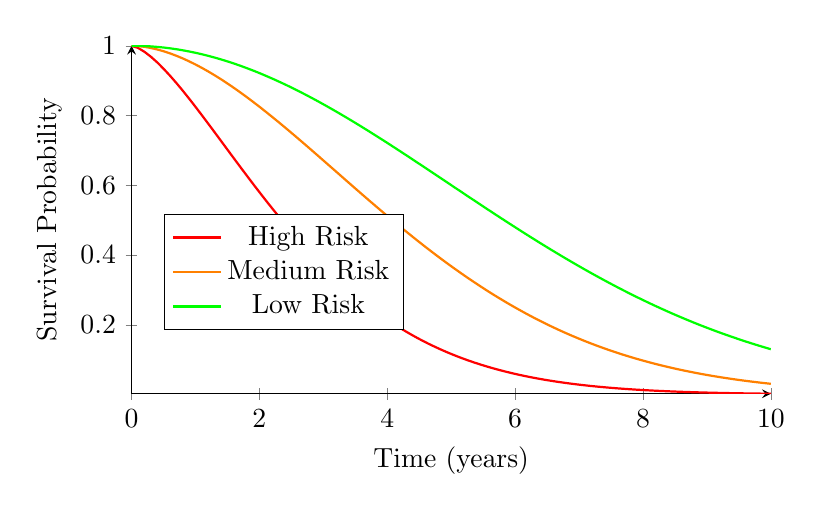
\begin{tikzpicture}
        \begin{axis}[
            width=0.8\textwidth,
            height=6cm,
            xlabel={Time (years)},
            ylabel={Survival Probability},
            axis lines=left,
            domain=0:10,
            samples=100,
            legend style={at={(0.05,0.35)}, anchor=west},
            ]
            % High risk group
            \addplot[red, thick] {exp(-(x/3)^1.5)};
            % Medium risk group
            \addplot[orange, thick] {exp(-(x/5)^1.8)};
            % Low risk group
            \addplot[green, thick] {exp(-(x/7)^2.0)};
            \legend{High Risk, Medium Risk, Low Risk}
        \end{axis}
    \end{tikzpicture}
    \caption{Risk stratification using DSM for breast cancer patients. The model identifies distinct risk groups with different survival trajectories, enabling more personalized treatment planning.}
    \label{fig:risk-stratification}
\end{figure}

\section{Summary: DSM in the Bigger Picture}

Deep Survival Machines represents a significant advance in survival analysis, bridging the gap between traditional statistical methods and modern deep learning approaches.

\subsection{Key Contributions}

\begin{itemize}
    \item Combines neural networks with parametric survival distributions
    \item Models complex hazard shapes through the mixture approach
    \item Provides natural uncertainty quantification
    \item Bridges the gap between deep learning and survival analysis
    \item Enables personalized risk prediction with confidence intervals
\end{itemize}

\subsection{Future Directions}

The DSM framework opens several exciting avenues for future research:
\begin{itemize}
    \item Integration with causal inference frameworks
    \item Extension to interval censoring and competing risks (MENSA)
    \item Combination with advanced embedding techniques for different data modalities
    \item Application to federated learning settings for privacy-preserving analysis
    \item Incorporation of domain-specific prior knowledge to enhance predictions
\end{itemize}

\begin{notebox}[title=Looking Ahead]
In the next chapter, we will explore Multi-Event Neural Survival Analysis (MENSA), which extends the DSM framework to handle competing risks scenarios where subjects can experience different types of events. MENSA addresses the challenge of modeling dependencies between different event types while maintaining the flexibility and power of the DSM approach.
\end{notebox}